%%% Introduction:
This section is designed to calculate correlation (or cross-correlation) among stock prices. Therefore, the Pearson product-moment correlation coefficient, denoted as $r$, will be calculated for each pair of stock prices:

\newcommand{\return}[1]{r_#1^{(t)}}
\newcommand{\returnt}[2]{r_#1^{(#2)}}
\newcommand{\stock}[1]{s_#1^{(t)}}
\newcommand{\stockt}[2]{s_#1^{(#2)}}
\newcommand{\stockmean}[1]{\bar s_#1}

\begin{align}
    r = \frac{\sum _{t=1}^{n} (\stock{i} - \stockmean{i})(\stock{j} - \stockmean{j})}{\sqrt{\sum _{t=1}^{n} (\stock{i} - \stockmean{i})^2 }  \sqrt{\sum _{t=1}^{n} (\stock{j} - \stockmean{j})^2 }}
    \label{formula:pearson_r} \\ \eqname{Pearson's $r$}
\end{align}

where $\stock{i}$ and $\stock{j}$ are the preprocessed stock prices of two companies at trading day $t$ and $n$ is the sample size. $\stockmean{i}$ and $\stockmean{j}$ are the sample means.

Unfortunately, stock prices produce time series comprising characteristics like autocorrelation and heteroscedasticity which distort the results of statistical inference (Section~\ref{subsection:bg-statistics}). The analysis of economic variables, better known as econometrics, originated from the application of statistical methods on financial time series and deals with such problems to discover models and relationships among economic variables. To avoid spurious correlation \cite{Yule1926WhyTime-Series} and conclude with meaningful cross-correlation coefficients, this analysis conducts prewhitening methods from econometric and time series analysis on the collected stock prices.

For applying our analysis including hypothesis tests and regression models, we use the implementations by the python modules \emph{scikit-learn} \cite{Pedregosa2011Scikit-learnPython} and \emph{statsmodels}.

\subsection{Data Processing}
\label{subsection:data_processing}
% https://drive.google.com/file/d/18l7y9Oh9uEo6yANFsUDggIIaOPDYqsR1/view

In the following, the stock prices will be transformed to account for preconditions of correlation analysis since it requires independently and identically distributed (i.i.d.) samples \cite{Franke2010StatisticsMarkets}. The most important of those are not existing autocorrelation (also known as serial correlation) and homoscedasticity but also other constraints which will be examined after the data was fully processed. In the last preprocessing step, autoregressive models will be conducted to deal with remaining autoregressive patterns.

% MOVE TO AR: Before applying regression on time series, multiple characteristics need to be examined in advance since they can distort the results.
% In order to achieve a stationary variable, the original data is differenced vanishing the unit root.
% Autocorrelation can arise in various forms, e.g. unit root, trend-stationary or moving-average processes

\subsubsection{Stationarity}
\label{subsubsection:processing:stationarity}
Time series reveal roots which indicate the dependency on previous values. If the influence of such a root persists over time and prevents the series to return to a stationary mean, this root is called a unit root \cite{Engle1987Co-IntegrationTesting} and the series is designated non-stationary. Stock prices are assumed to contain a unit root \cite{LopezdePrado2018AdvancesLearning} which can be accounted for by differencing the time series. Depending on the data one uses, this can be done by taking the absolute or relative differences between each sample:

\begin{align}
    \Delta_i^{(t)} &= c_i^{(t)} - c_i^{(t-1)} \label{formula:abs_diff} \\ \eqname{Absolute Difference} \\
    \Delta_i^{(t)} &= \frac{c_i^{(t)}}{c_i^{(t-1)}} \label{formula:rel_diff} \\ \eqname{Relative Difference}
\end{align}

where $c_i^{(t)}$ is the unmodified closing stock price at trading day $t$.

To have comparable measures among stocks with different levels, the relative difference is used hereinafter. The selected dataset provides the open, close, high and low stock prices for each day so there are various ways to create returns, i.e. differences of the daily stock prices. \citet{Hong1998TradingClosures} provides empirical findings about recurring patterns in returns including that open-to-open returns are more volatile than close-to-close returns. \citet{Wang2009StatisticalReturn} provide evidence that intraday (open-to-close) and overnight (close-to-open) returns have significantly different properties concluding that one shall not mix them. \citet{Li2014NewsAnalysis} considers daily open-to-close prices arguing that it is less prone to seasonality and the more volatile non-trading gaps across weekends and holidays. 

The skewness and kurtosis of the current data investigated supports these findings. The distributions of open-to-open and close-to-close returns reveal a high kurtosis, conforming with related work that stock prices are leptokurtic \cite{Morgan1976StockHeteroscedasticity}. For the overnight returns extremely high kurtosis is observed upon the data used in this work. In contrast, the kurtosis of intraday returns is approximately three which equals the kurtosis of a normal distribution. For the skewness, we see a similar behaviour. The overnight returns revel a large negative skewness. While open-to-open and close-to-close returns substantiate a moderate negative skew (-0.1 in average) coinciding with related work, the intraday returns are distributed with a slightly positive skew (0.06 in average). Because of their more normal like distributions, intraday returns are used in the following which are calculated by the formula in Eqn.~\eqref{formula:return}. From a theoretical point of view, it is even more intelligible to select the returns across the period during high activity on the market. The returns are more likely to represent the impact of actual news and therefore reach faster a stable price level.

\begin{align}
    r^{(t)}_i &= \frac{c^{(t)}_i}{o^{(t)}_i}
    \label{formula:return} \\ \eqname{Intraday Return}
\end{align}

where $o_i^{(t)}$ and $c_i^{(t)}$ are the open and close prices for a stock at trading day $t$.


\subsubsection{Homoscedasticity}
\label{subsubsection:processing:homoscedasticity}
Another precondition for correlation is homogeneous volatility (variance in the context of time series), in the following denoted as homoscedasticity. The lack of this property is called heteroscedasticity. Unfortunately, stock prices are assumed to be heteroscedastic \cite{Morgan1976StockHeteroscedasticity}. In most cases, this can be addressed by modelling the time series with a generalized autoregressive conditional heteroscedasticity
(GARCH) model, using heteroscedasticity-consistent standard errors (e.g. Newey-West estimator) \cite{Millo2017RobustApproach} or applying robust regression methods (e.g. weighted least squares regression). If this not handled in any way, most test statistics tend to report biased results, e.g. the method of ordinary least squares (OLS) is not anymore the best linear unbiased estimator resulting in downwards biased coefficients \cite{Hallin2014Gauss-MarkovStatistics}. Usually, there can be various reasons for observing heteroscedasticity. For example. sensor data or data extracted from very noisy sources, such as text, may reveal measurement errors. In the context of stock prices, the heteroscedasticity is most likely caused by leaving out exogenous factors which will be treated in the following step of preprocessing.

% https://mpra.ub.uni-muenchen.de/54954/1/MPRA_paper_54954.pdf
% "Some statistical tests, for example the analysis of variance, assume that variances are equal across groups or samples. The Levene test can be used to verify that assumption."


One popular method for heuristic data stabilization is the Box-Cox transformation \cite{Box1964AnTransformations}. It is a simple power transformation which is applied on the calculated returns \eqref{formula:boxcox} to stabilize the data. It is assumed to mitigate heteroscedasticity, which will be examined in a later section. As suggested by \citet{Box1964AnTransformations}, the model's power parameter $\lambda$ is determined by maximizing the log-likelihood function.

\begin{align}
    r_i^{(t)(\lambda )} &={\begin{cases}{\dfrac {r_i^{(t)^\lambda}-1}{\lambda }}&{\text{if }}\lambda \neq 0,\\ \quad \ln r^{(t)}_i&{\text{if }}\lambda =0,\end{cases}}
    \label{formula:boxcox} \\ \eqname{Box-Cox Transformation}
\end{align}

where $r_i^{(t)(\lambda )}$ is the intraday return for a stock price at trading day $t$ after it was slightly adapted by a Box-Cox transformation with power parameter $\lambda$. In the following this transformed return is denoted as $r_i^{(t)}$ doe simplicity.


\subsubsection{Exogenous Variables}
\label{subsubsection:processing:exogenous}

As stated in the beginning of this study, financial markets are prone to manifold external influences which are usually not modelled during regressing stock prices. This type of mis-specification of leaving out exogenous variables in models is quite common, because they can not be observed directly or their inclusion increase the problem space in an excessively manner. Therefore, economic models usually focus on a few variables which are of high interest.

To account for those exogenous variables data normalization regarding the overall market behaviour is carried out. If the economy is doing well or experiences a period of uncertainty, this will be likely reflected in all stock prices. The selected stock prices are even part of the market index reflecting the overall market performance. Hence, omitting exogenous variable is another reason for spurious correlation \cite{Granger1969InvestigatingMethods}. A greater correlation between stock prices can be caused by a shared external factor which is the common market performance in this case. To have a better representation for the performance of a single stock, its returns needs to be normalized regarding the shared performance of the market. Further, the underlying movement of a stock price might even more be biased by the sentiment of the according industry section. Stocks from the same industry will therefore have a high cross-correlation without revealing a specific relationships, caused by the similar behaviour of investors in this section of the market.

In the following, the return value will be subtracted by the average return value of its industry sector:

\begin{align}
    \hat r^{(t)}_i &= r^{(t)}_i - \frac{1}{|B_{j}^{(t)}|} \sum \limits_{r^{(t)}_k \in B_{j}^{(t)}} r^{(t)}_k
    \label{formula:normalization} \\ \eqname{Industry Normalization}
\end{align}

where $B_{j}^{(t)}$ is a set of the transformed intraday returns at trading day $t$ for all companies in the same industry sector as the company for $r^{(t)}_i$. The resulting normalized intraday return $\hat r^{(t)}_i$ will be denoted in the following as $r^{(t)}_i$.


Normalizing by the S\&P~500 market index instead of the separate industry means will be examined by the distribution of resulting cross-correlations in Section~\ref{subsection:cross_correlation}.
\subsubsection{Autoregression}
\label{subsubsection:processing:ar_modelling}

Even though, differencing and normalization successfully remove some autocorrelations, autoregressive patterns can remain which can be accounted for by autoregressive models. In contrast to their most popular application (e.g. \citet{Ruiz2012CorrelatingActivity}), autoregressive models are not used for forecasting purposes. They are simple linear models with unrealistic constraints and thereby far exceeded by machine learning models \cite{Hsu2016BridgingEconomists}. Nevertheless, they are able to model the linear autoregression of time series which shall be filtered out before cross-correlating time series. If a temporal variable reveals autoregression, a value within this time series can be described by a function of its past values plus an error term $\epsilon$ which is also known as residual. If such autoregression is present for two correlated time series, the calculated correlation coefficient is found to be invalid. Instead, a suitable autoregressive model shall be applied and correlation analysis conducted on the residuals because they are assumed to be free from linear autoregression.

% "Regression models for prediction are often useful even when the assumptions are moderately violated, although they may not perform optimally. However, in many applications, especially with small effects or questions of causality based on observational data, regression methods can give misleading results.[2][3]" (https://en.wikipedia.org/wiki/Regression_analysis)

% History of Time Series Analysis, Types of interventions (omitted vars.), etc. --> https://autobox.com/cms/index.php/afs-university/intro-to-forecasting/doc_download/1-the-autobox-advantage

\paragraph{ARMA}
To remove autoregressive patterns in the mean of the process, an autoregressive-moving-average (ARMA) model is applied \cite{Dionisio2004MutualSeries}. It assumes a temporal observation to be linear combination of the $p$ lagged values and the $q$ lagged error terms from the same stationary and univariate time series \eqref{formula:ar_model}. The remaining value, in the following residual, which cannot be modelled by these terms is called the error term and is assumed to be i.i.d. It should not reveal any significant autocorrelation if an appropriate ARMA model was selected and therefore is valuable for further correlation analysis avoiding spurious correlation \cite{Yule1926WhyTime-Series}. A common approach for determining the hyper parameters, known as Box-Jenkins method \cite{Box1970TimeControl}, uses the autocorrelation function (ACF) and partial autocorrelation function (PACF) \cite{Franke2010StatisticsMarkets}. The ACF describes the correlation of an observation with lag values. The PACF has the same focus but uses a statistically adjusted correlation that is not accounted for by intermediate lags. For the model identification, the number of significant correlation lags from the PACF determines $p$ while the number from the ACF determines $q$. The resulting model is denoted as ARMA(p, q).

% https://machinelearningmastery.com/gentle-introduction-autocorrelation-partial-autocorrelation/
% https://ncss-wpengine.netdna-ssl.com/wp-content/themes/ncss/pdf/Procedures/NCSS/The_Box-Jenkins_Method.pdf
% https://www.academia.edu/2099523/Time_series_analysis_forecasting_and_control
% https://machinelearningmastery.com/gentle-introduction-box-jenkins-method-time-series-forecasting/

\begin{align}
    \returnt{i}{t} &= \sum \limits_{j=1}^{p} a_j \returnt{i}{t-j} + \sum \limits_{j=1}^{q} b_j \epsilon_{t-i} + \epsilon_t  \label{formula:ar_model} \\ \eqname{ARMA Model}
\end{align}

The intraday return at $t$ is regressed by $p$ lagged values $\returnt{i}{t-p}, ..., \returnt{i}{t-1}$ and $q$ lagged error terms $\epsilon_{t-q}, ..., \epsilon_{t-1}$. In order to do so, the model coefficients $a_1, ..., a_p$ and $b_1, ..., b_q$ are fitted with OLS. $\epsilon$ denotes the residual representing the part of $\returnt{i}{t}$ which can not be described by autoregression and therefore is considered to be free of autocorrelation. In the following, the model residual is denoted with $\returnt{i}{t}$. It also involves those stock returns for which no autoregressive modelling was required.

\begin{figure}[!ht]
    \centering
    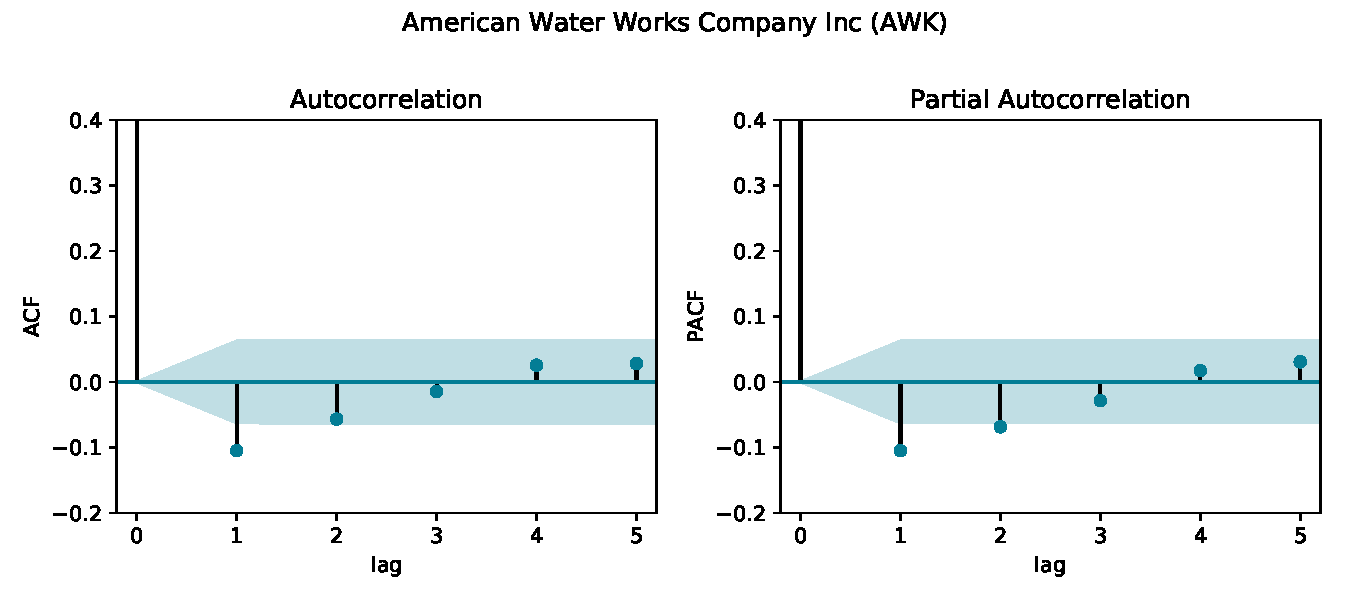
\includegraphics[width=\textwidth]{figures/regression/acf-awk-normed.pdf}
    \caption{ACF and PACF plots for the preprocessed stock returns for company \emph{American Water Works Company Inc}. The x-axis shows the lag and the y-axis shows the correlation coefficient (Pearson's $r$). The colored area around zero represents the 0.95 confidence interval of no significant correlation. All values out of this range can be assumed to be correlated. The autocorrelation of a zero lag will always be one, so the plots are adjusted to not fully show this dispensable data point but put more focus on the following lags.}
    \label{fig:acf_pacf_awk_normed}
\end{figure}

For 385 stocks there was no autocorrelation observable so the ARMA model was not applied on this data. To show an example how lags are determined and how the modelling reduces autocorrelation, the ACF and PACF are plotted in Figure~\ref{fig:acf_pacf_awk_normed} for an example company. The ACF shows significance for one lag while the PACF even shows significance for two lags, so an ARMA(2, 1) model will be applied.

\begin{figure}[!ht]
    \centering
    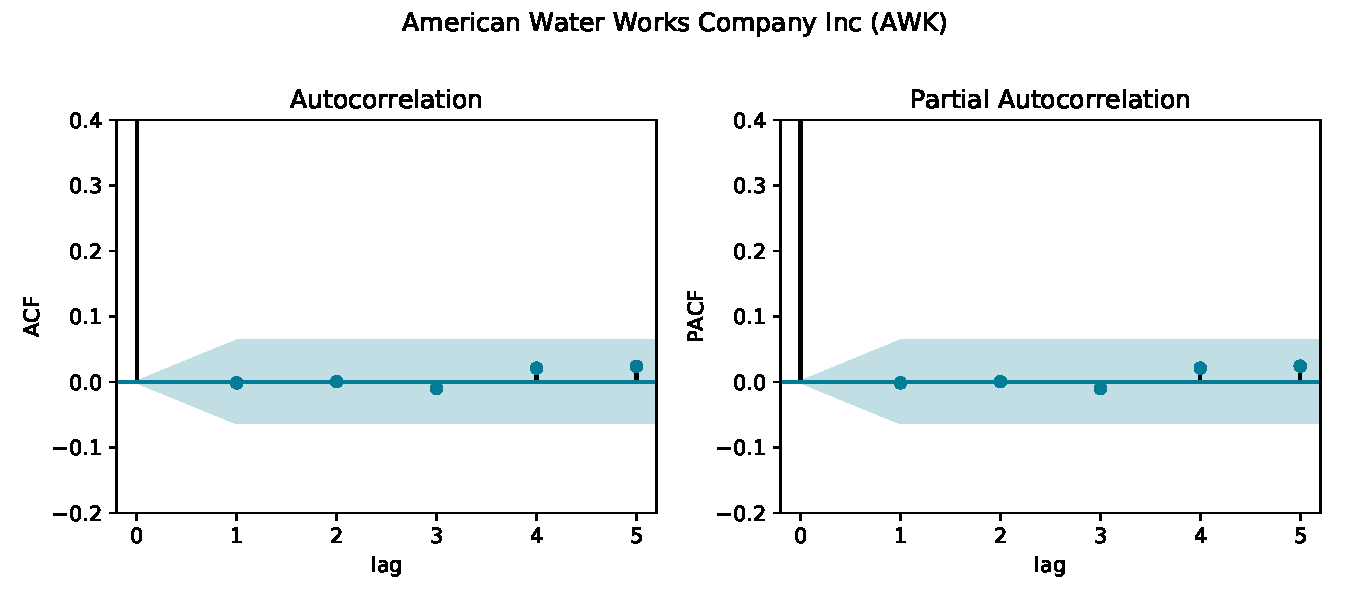
\includegraphics[width=\textwidth]{figures/regression/acf-awk-resid.pdf}
    \caption{ACF and PACF plots for the preprocessed stock returns for company \emph{American Water Works Company Inc} after taking the residuals of an ARMA(2, 1) process.}
    \label{fig:acf_pacf_awk_resid}
\end{figure}

Figure~\ref{fig:acf_pacf_awk_resid} shows the same plots for ACF and PACF after the autoregressive process was filtered out. There is no significant autocorrelation left, so the modelling was successful. To inspect the outcome of this modelling, later evaluation will investigate the autocorrelation of residuals extracted from those ARMA models. If no model was applied because it was not appropriate, the time series is still treated as the residuals of a mean process justifying the usage of the following model for volatility.

\paragraph{GARCH} In the last step of preprocessing, the autoregressive patterns in volatility are modelled which needs to be done additionally to the previous mean modelling by ARMA models. The generalized autoregressive conditional heteroscedasticity (GARCH) model \cite{Bollerslev1986GeneralizedHeteroskedasticity} is a way to treat the unstable volatility in stock prices which are already assumed to be not mean autocorrelated, stationary and without structural breaks. It is applied on the residuals of a mean process which resulted from the previous ARMA(p, q) modelling. The GARCH(u, v) model approximates the residual's volatility $\sigma^2(t)$ (standard deviation over time) by a linear combination of $u$ previous volatility values and $v$ previous residuals, as shown in formula~\eqref{formula:garch_model}: % The parameter $\omega$ denotes the constant volatility over the whole process.

\begin{align}
    {\sigma_i^{(t)}}^2 &= \sum \limits_{j=1}^{v} c_j {\returnt{i}{t-j}}^2 + \sum \limits_{j=1}^{u} d_j {\sigma_i^{(t-j)}}^2 + \omega \label{formula:garch_model} \\ \eqname{GARCH Model}
\end{align}

where $\omega$ is the constant volatility over the whole time series, $\returnt{i}{t-v}, ..., \returnt{i}{t-1}$ are the considered residuals of the previous ARMA model and ${\sigma_i^{(t)}}^2$ is the volatility of $\returnt{i}{t}$ at trading day $t$. The model coefficients for incorporating lagged residuals and volatility are $c_1, ..., c_v$ and $d_1, ..., d_u$.

For estimation of the hyper parameters $u$ and $v$ of a GARCH(u, v) model, a similar method as for ARMA(p, q) is conducted on the squared residuals which are supposed to be zero-mean. Because the actual volatility cannot be directly observed, the squared residuals are commonly used as a proxy. Depending on the number of lags of significant (partial) autocorrelation, $u$ and $v$ are chosen. % There are other approaches for determining parameters of a GARCH model like using an Information Criterion which measures the suitability of model.

To conclude with homoscedastic data for the following correlation analysis, the standardized residuals are calculated from this model by dividing the previous ARMA residuals by the conditional volatility calculated with the GARCH model, as shown in Formula~\eqref{formula:std_resid}. The stocks, for which no GARCH model was applied, are divided by their overall standard deviation to keep the time series in the same scale. It is important to mention that this will not affect the results since the same scalar is used for all values of the time series.

\begin{align}
    \stock{i} &= \frac{\return{i}}{\sigma_i^{(t)}}
    \label{formula:std_resid} \\ \eqname{Standardized Residuals}
\end{align}

where $\stock{i}$ is the final variable which will be used in the following for time series analysis. It incorporates both model residuals and rectified intraday returns depending on whether a model was applied or not.

\begin{figure}[!ht]
    \centering
    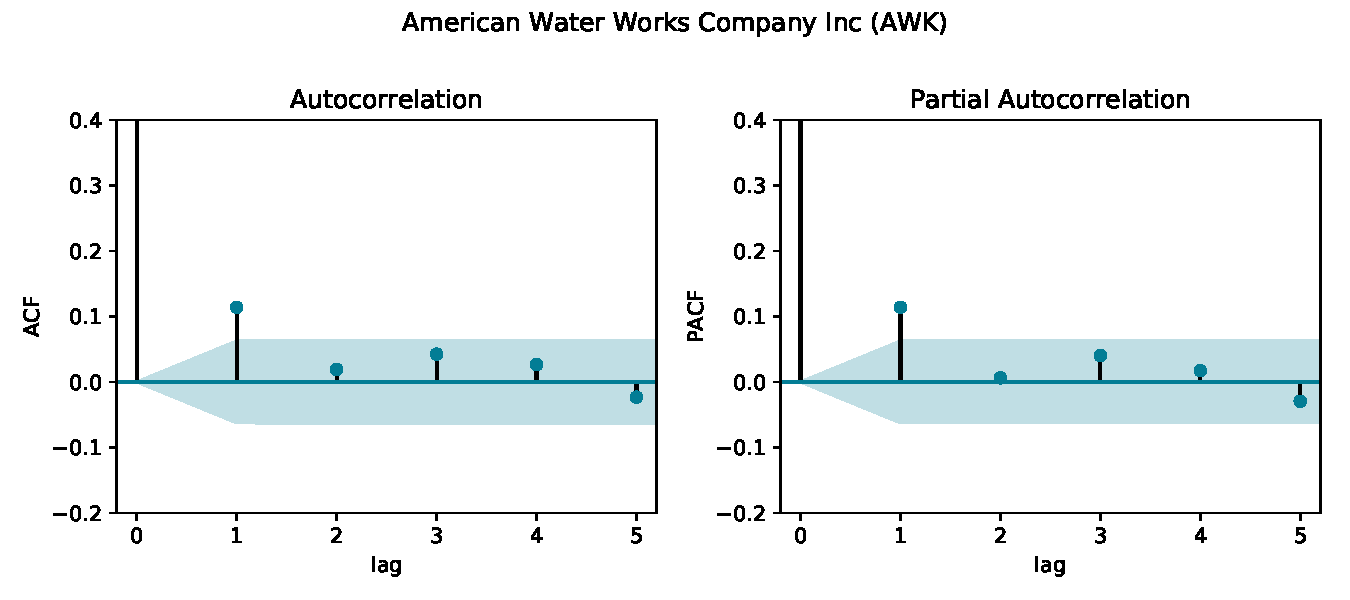
\includegraphics[width=\textwidth]{figures/regression/acf-awk-resid-sqr.pdf}
    \caption{ACF and PACF plot for the squared residuals after applying a ARMA(2, 1) model on the preprocessed stock returns for company \emph{American Water Works Company Inc}.}
    \label{fig:acf_pacf_awk_resid_sqr}
\end{figure}

Figure~\ref{fig:acf_pacf_awk_resid_sqr} visualizes the ACF and PACF for the approximated volatility of an example company by using its squared preprocessed stock returns. The ACF and PACF both reveal significance for the first lag only. This leads to the suggestion of applying a GARCH(1, 1) model.

\begin{figure}[!ht]
    \centering
    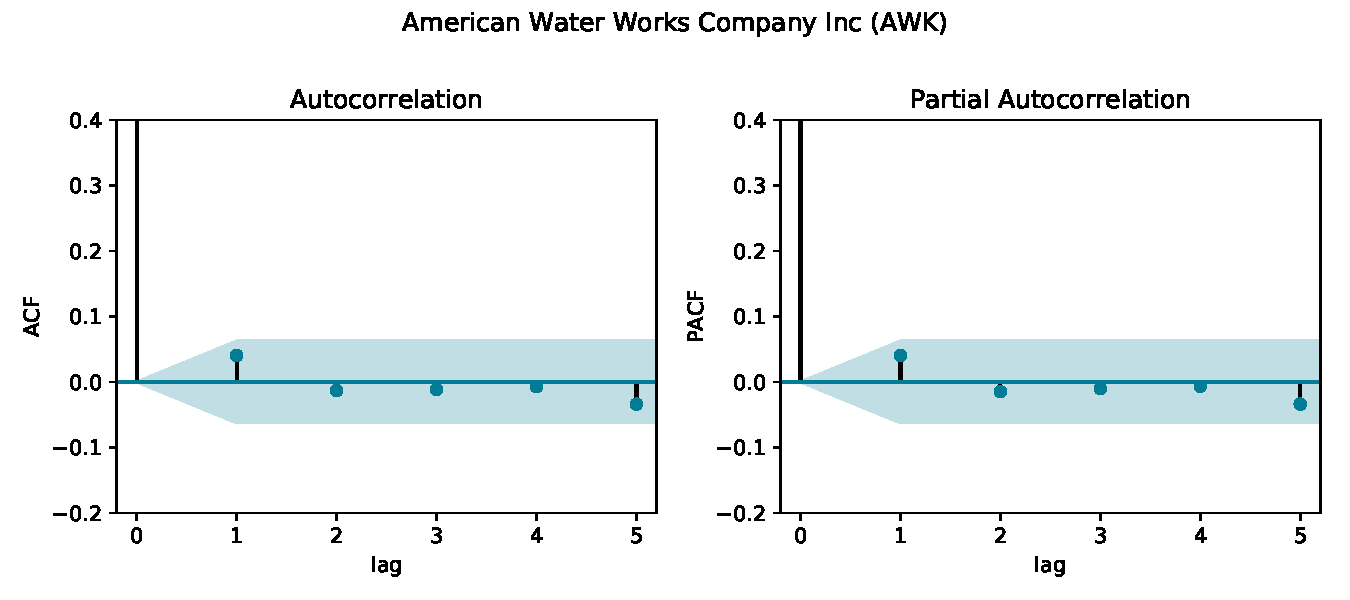
\includegraphics[width=\textwidth]{figures/regression/acf-awk-std-resid-sqr.pdf}
    \caption{ACF plot for the squared residuals after applying a ARMA(2, 1) and a GARCH(1, 1) model on the preprocessed stock returns for company \emph{American Water Works Company Inc}.}
    \label{fig:acf_pacf_awk_std_resid_sqr}
\end{figure}


To evaluate the success of the approach, the ACF and PACF of the standardized residuals are shown in Figure~\ref{fig:acf_pacf_awk_std_resid_sqr}. Clearly, the autocorrelations of the considered lag and even some following lags diminished to a insignificant level close to zero. Under the same procedure, the need of modeling volatility and selection of suitable hyper parameters is examined on all 467 stocks. For 306 from these a GARCH model is applied, usually with $u=1$ and $v=1$.



% The autoregressive–moving-average (ARMA) modelling requires stationarity for calculating its slope coefficients. They are usually calculated using Ordinary Least Squares (OLS) \cite{GrangerNewbold}.


% FORECAST WITH FEASIBLE MODELS: Based on the previously found properties select model (LR, ARIMA, EGARCH, GARCH, etc.). Evaluate models with MAPE (include Diebold and Mariano (DM) test?) and information criterion (AIC, BIC, HCQ). (parametric: ARIMA vs. non-parametric: Link relatives, difference)
%   A) ARIMA parameters can be estimated by finding last significant lag in ACF & PACF. Afterwards evaluate by inspecting "Residual vs fitted" chart and ACF of the models residuals https://newonlinecourses.science.psu.edu/stat510/node/47/
%   B) For predictions: persistence model as baseline

% \subsubsection{Exogeneous Variables}
% Taking GSPC & industry into account as exogeneous variables enables us to reflect other external influences which have an impace on the whole market.


\subsection{Time Series Evaluation}
\label{subsection:time_series_evaluation}
After the stock prices were differenced, stabilized, normalized and autoregressively modeled, characteristics of the resulting time series will be examined. While there are easy to apply methods for establishing stationarity and removing trends, some characteristics like structural breaks are most likely hard to remove. Therefore, in some cases not all preconditions are ensured. But the data is not further transformed to enforce less outliers, removed periodicity or ensure ergodicity. By applying yet another transformation in order to achieve those conditions, the data might be polluted in a too drastic way. However, one should be aware of the level of violations for assumptions which are required in correlation analysis.

\begin{figure}
    \centering
    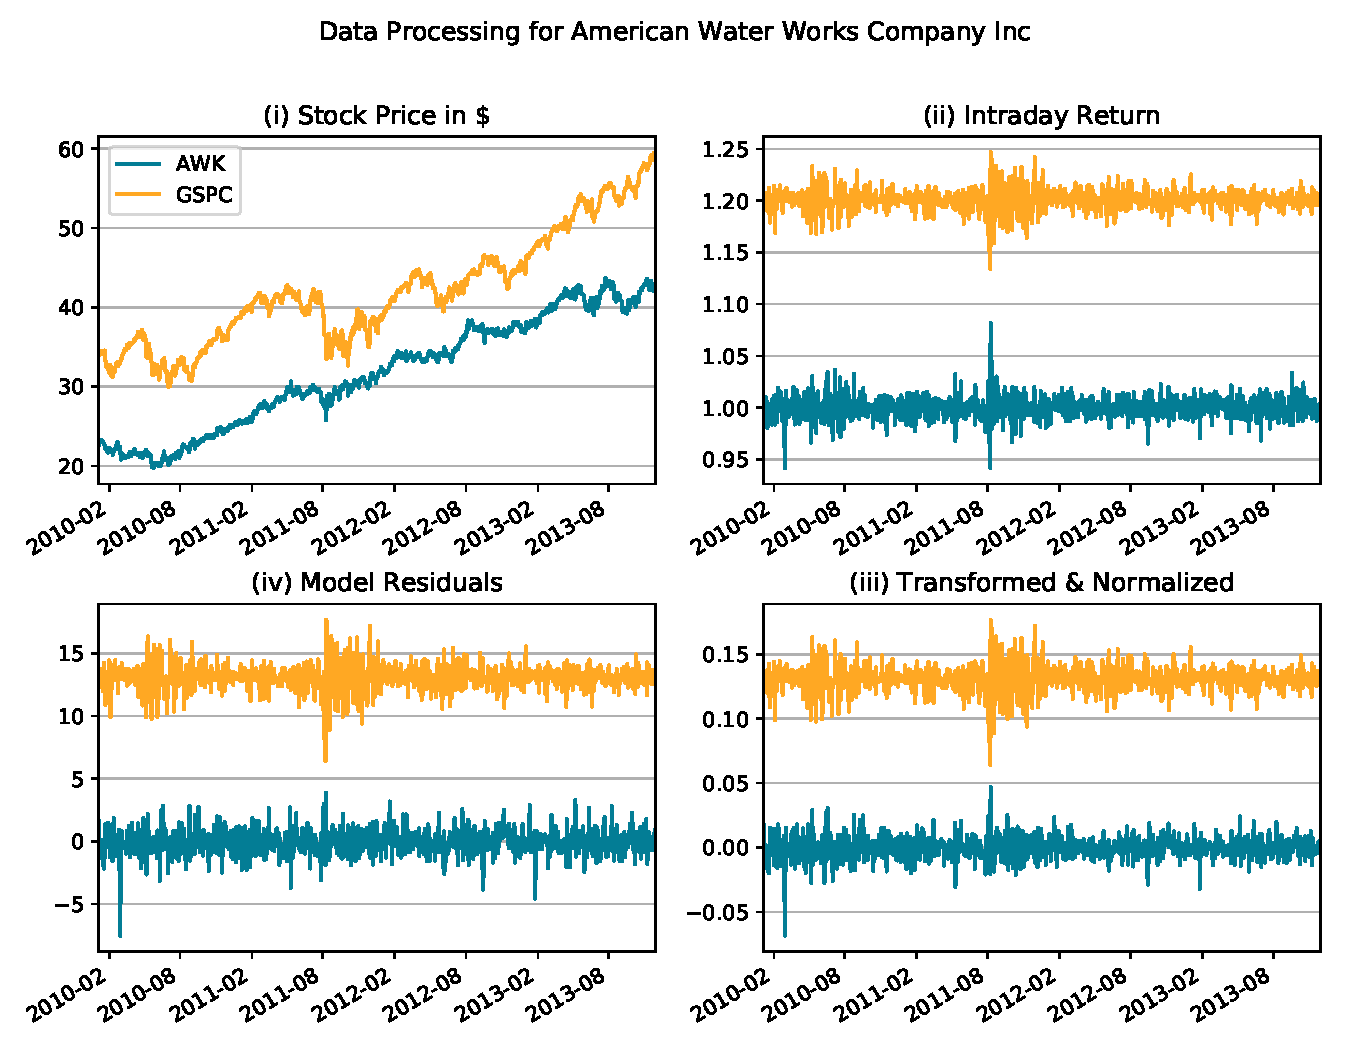
\includegraphics[width=0.9\textwidth]{figures/regression/data-processing-awk.pdf}
    \captionsetup{singlelinecheck=off}
    \caption[foo bar]{Values from intermediate preprocessing steps for the company \emph{American Water Works Company Inc} are shown in blue and compared with the price or intraday return of the S\&P~500 market index in orange. In all cases, the index was scaled and shifted in order to show both time series next to each other. The preprocessing steps are arranged clockwise, starting from the top left corner: \begin{enumerate*}[label=(\roman*)]
        \item unmodified stock prices,
        \item intraday returns,
        \item stabilized and industry-wise normalized returns and
        \item standardized residuals of ARMA(2, 1) and GARCH(1, 1) models on returns.
    \end{enumerate*}}
    \label{fig:data-processing-steps}
\end{figure}

Figure~\ref{fig:data-processing-steps} visualizes the impact of preprocessing on a stock price and takes the S\&P~500 market index into account. In the first plot both time series move strongly similar. After taking the intraday returns, stationarity appears to be ensured but both time series still tend to reveal similarity, e.g. by simultaneous bursts or change in volatility. Subsequently, the return values are stabilized with Box-Cox transformation and normalized by the regarding industry mean. Even though some parts still indicate an existing relationship, the time series is located more stable around zero and reveals less outlier. In the last step, the volatility is adjusted by ARMA and GARCH modelling, resulting in a time series which appears to be very similar to a white noise. Since a white noise process is considered to fulfill almost all constraints in order to be i.i.d., the data seems to be promising for further analysis.


\subsubsection{Stationarity}
\label{subsubsection:stationarity}

The stationarity is one of the most important properties one need to examine before conducting further time series analysis. If it is not present, experiments like correlations or ARMA models lead to falsely results. The stationarity is evaluated by applying hypothesis tests for the presence of unit roots on the examined time series. It is recommended to apply multiple hypothesis tests to provide assurance of a correct outcome, so we will execute the following ones:
\begin{enumerate*}[label=(\roman*)]
    \item Augmented Dickey-Fuller (ADF) \cite{Dickey1976IntroductionSeries}
    \item Phillips-Perron (PP) \cite{Phillips1988TestingRegression}
    \item Kwiatkowski–Phillips–Schmidt–Shin (KPSS) \cite{Kwiatkowski1992TestingRoot}
\end{enumerate*}

The first two test the null hypothesis, that a unit root is present. In contrast, the latter one tests the null hypothesis of stationary data. As common practice (e.g. \cite{Bishara2012TestingApproaches}), the significance level $\alpha=0.05$ is defined for the $p$-value in order to sufficiently reject the null hypothesis.

All three tests are executed on all 467 stock prices at each step of their preprocessing stage. Except for 14 cases, all three tests attest the presence of a unit root in the original stock prices. After taking the intraday returns, there is no stock, for which all three tests simultaneously give evidence for a unit root. Only the KPSS test significantly rejects the absence of unit roots for 15 cases. The following preprocessing steps did not change this number by large, so the final time series can be expected to be stationary.

% "Any series that has a trend will tend to be correlated to any other series that has a trend. For this reason, it is preferable to remove trends and seasonal effects before comparing multiple series. This is usually achieved by working with the residuals of a fitted time series model, such as the regression models of Chapter 3" (Introductory Time Series With R, Cowpertwait and Metcalfe )

% "The model should only be applied to a prewhitened residual series {e_t} that is uncorrelated and contains no trends or seasonal changes, such as might be obtained after fitting a satisfactory SARIMA model." (Cowpertwait and Metcalfe, Page 148, Introductory Time Series with R, 2009)

% RESOLVE unit root: If it cannot be rejected one may run the same test after applying a difference operator like AR(1), AR(2) or Link relatives.
% Diagnostic checking on residuals for:
%   A) Normality 
%   B) Autocorrelation 
%   C) Het.Sce. 
%   D) Test for structural breaks?
%   E) Other properties like periodicity, seasonality and outliers

% Even though there are a lot of factors influencing the stock markets behaviour one needs to cut it down to a few more important variables. Omitting influencing exogeneous factors might lead to spurious correlations / endogeneity but we need to reduce the dimensions of freedom avoiding curse of dimensionality (what is endogeneity: https://www.statisticshowto.datasciencecentral.com/endogenous-variable/) -> Check for endogeneity (error term correlates with independent variable within the model). This would mean that the model is biased and regression analysis using OLS is erroneous. Possible reasons for endogeneity: ommited variables; Measurement error in variable (noise is considered to be part of variable) -> OLS estimation will be biased downwards; Simultaneity (fixed by Instrumental Variables Regression)

% UNIT ROOT: Is it unit root? (explained in background) Apply ADF, PP and/or KPSS as \cite{Vlastakis2012}. Differentiate between trend-stationary, difference-stationary and just non-stationary. If and only if the null hypothesis of unit root can be rejected, one can apply autoregression; "A finding of a unit root implies that stock returns cannot be predicted." \cite{Narayan2005}. Unit root processes are tíme-series which do not fully recover from shocks. The term originates from a coefficient equal to one for the last value when the next value is calculated, hiding/covering the underlying trend ones is looking for.


\subsubsection{Data Distribution}
\label{subsubsection:normal_dist}

% Many financial variables are non-normally distributed (Mandelbrot and Benuit 1963)

Another precondition of cross-correlation are normal distributed samples \cite{Bishara2012TestingApproaches}. For evaluating if the data distribution is similar to a normal distribution, again hypothesis tests are a good way to acquire evidence in favour of or against normality being present. For example, \citet{Vlastakis2012InformationVolatility} use the Jarque-Bera test \cite{Jarque1980EfficientResiduals} to inspect the null hypothesis that a normal distribution is present. Conducted on the 30 stocks from Dow Jones Industrial Average, they reject the presence of a normal distribution with 99~\% confidence. As stated in the previous section, it is a common practice to use multiple tests for double-checking the results. For this task, the following are applied which all rely on the same null hypothesis of normality being present:
\begin{enumerate*}[label=(\roman*)]
    \item Jarque-Bera (JB) \cite{Jarque1980EfficientResiduals}
    \item Shapiro-Wilk (SW) \cite{Shapiro1965AnSamples}
    \item D’Agostino’s K\^2 (DK2) \cite{DAgostino1973Testsb}
    \item Anderson-Darling (AD) \cite{Stephens1974EDFComparisons}
\end{enumerate*}

As might be expected from the initial analysis of kurtosis and skewness in Section~\ref{subsubsection:processing:stationarity}, only 16 out of 467 preprocessed stock prices reveal evidence for a normal distribution by at least one test statistic.


To inspect the possibility of another distribution, the Kolmogorow-Smirnow (KS) \cite{Massey1951TheFit} test is applied. It assesses the equality of two distributions by calculating the distance of their cumulative distribution function. The distributions of each preprocessed stock prices is compared to a set of common probability distributions. The most frequently distribution (using a rejection rate of $\alpha=0.05~\%$) was Student's $t$ with 7 dimensions of freedom in average, followed by logistic, laplace and normal distribution. Based on the suggested distributions, the data appears to have heavier tails as a normal distribution. % Still, the normal distribution appears to be a reasonable assumption for 304 out of 467 preprocessed stock return series and the close average kurtosis and skewness provide evidence for the suitability. Except for the examination of outliers, the data will therefore be treated as a normal distribution.

These findings do not lead to the conclusion that calculating the correlation on such non-normal data returns erroneous conclusion. The Pearson correlation coefficient, which will be introduced later, is fairly robust for different data distributions, although it does assume normality. Only if the distribution differs strongly from normality, e.g. by extreme values for skew or kurtosis, it should be treated with caution \cite{Bishara2012TestingApproaches}.

% https://sci-hub.se/10.2466/pms.1976.43.3f.1319


\subsubsection{Homoscedasticity}
\label{subsubsection:homoscedasticity}

Economic variables like stock prices are known to potentially exhibit heteroscedasticity \cite{Salisu2016UnitSeries}. To examine linear versions of heteroscedasticity, the Breusch-Pagan test (BP) \cite{Breusch1979AVariation} can be used. If this test fails to reject the null hypothesis of homoscedasticity and therefore indicates the presence of homoscedasticity, the White test \cite{White1980AHeteroskedasticity} can be applied to test for nonlinear forms. It checks the null hypothesis on a greater set of terms which needs more calculation and might reveal less significant results than BP. Because of the large number of degrees of freedom, the White test can over-react. Concluding, both tests are applied in the following. % https://www3.nd.edu/~rwilliam/stats2/l25.pdf

While at least one test indicated heteroscedasticity for 422 stocks based on their intraday return values, 307 remained with significant results after transformation and normalization. The enhanced stability in form of volatility, gives subsequent justification for the previous prewhitening steps. In more than a half of these cases the White test revealed sufficient evidence while the BP did not. This leads to the conclusion that in many cases the data contains nonlinear heteroscedasticity, which BP is not able to detect.

After applying the GARCH model, 28 stocks remain which do not satisfy both tests for homoscedasticity. Besides those 28 stocks, 94 stocks have at least one test showing evidence for rejecting the null hypothesis. Most of these show evidence for the White test. Since this leads to the conclusion that there is still nonlinear heteroscedasticity present, the GARCH model might be not the best model and a more sophisticated approach like a nonlinear GARCH might be more suitable in future work. However, a large proportion of heteroscedasticity was removed compared to the original stock returns.

% (White Test with stats.diagnostic.het_white [from https://machinelearningmastery.com/develop-arch-and-garch-models-for-time-series-forecasting-in-python/)], BP test including the squared value, Engle's ARCH test (null=homo), Levene's Test -> https://sci-hub.se/10.2307/2328672) 

% (https://www.researchgate.net/post/How_to_remove_serial_correlation_and_heteroskedasticity) (https://mpra.ub.uni-muenchen.de/54954/1/MPRA_paper_54954.pdf) (https://sci-hub.se/10.1080/00036840802600087)

\subsubsection{Structural Breaks}
\label{subsubsection:structural_breaks}

% Additionally, the following analysis inspects the time series on structural breaks like shifts or bursts, and heteroscedasticity (heterogeneous volatility) \cite{xxxSalisu2016}.

Regression models, which are broadly used for hypothesis testing and other purposes, are established by estimating the coefficient of regressors fitting the dependent variable. A big issue of such coefficients are their stability. If the regressed variables contain structural changes like a level shift in mean or volatility, the estimated coefficients are most likely to be not suitable. If a specific point of time should be examined regarding a structural break, tests can be used which compare the regression coefficients which are calculated separately on each half of the dataset. If the coefficients are sufficiently different from each other, the time series can be assumed to have a structural break at the chosen time stamp.

However, examining the existence of structural breaks in an unsupervised manner, i.e. at an unknown point of time, appears to be a more difficult topic. Even, the application of machine learning for unsupervised anomaly detection is an ongoing topic, which is not completely reliable. All the more, the automated check using a statistical approach should be viewed skeptical. Therefore, only evidence for the presence of an unknown number of structural breaks is collected. The work will not further deal with it, accepting their presence for a few cases. The CUSUM-test \cite{Brown1975TechniquesTime} can be used for these cases, testing the null hypothesis of stable coefficients of a linear regression model.

Only two out of all original stock prices are assumed to contain at least one structural break following the CUSUM-test. The number increases only slightly after differencing and normalization concluding with 22 stocks revealing unstable coefficients. Even though, we are trying to remove the mean movement across one industry, not all prices might contain this common behaviour for the entire period. For some stock prices, the normalization step appears to introduce a new movement sectionally which leads to the significant rejection of stable coefficients over the entire times series.

\subsubsection{Autocorrelation}
\label{subsubsection:autocorrelation}

To test the autocorrelation across the whole dataset, two hypothesis tests were applied. The Durbin-Watson statistic \cite{Durbin1971TestingRegression.III} returns a number between 0 and 4 with suggesting no autocorrelation for the first lag if the statistic falls between 1.5 and 2.5. The Ljung-Box Q Test \cite{Dionisio2004MutualSeries} was also applied on the first lag only and tests the null hypothesis of no autocorrelation. Before applying autoregressive models, the preprocessing already reduced the number of first-lag autocorrelated stock returns from 467 down to 82 which was also observed previously by looking at the significant lags of ACF and PACF in Section~\ref{subsubsection:processing:ar_modelling}. For these remaining cases, the modelling was applied and successfully cleared the autocorrelation completely for all time series.

\subsubsection{Further Properties}

Variables and their regarding distributions are hard to describe without visualizing the data. descriptive properties like skewness, kurtosis and heteroscedasticity are provided, but they can not fully reflect the data itself. Even though stationarity is validated, latent periodic patterns can still remain.

\paragraph{Seasonality} 
Following the decomposition model, some autoregressive patterns can be describes by seasonality (recurring at fixed time intervals) or cyclicality (recurring patterns without fixed time frames). Since the data preprocessing does not account for these properties, it needs to be conducted if there is evidence for such periodic patterns. Especially, daily prices are prone to seasonality in form of weekly, monthly or seasonal patterns. Since two stock prices might follow the same pattern, there is always a chance of falsely correlating stock prices. Related work suggests using a differencing window over a year, so only two days from the same time of a year are always compared. Despite of a sliding window, this would decrease the number of resulting data points by about 250 samples (number of trading days in one year) which is critical for the size of the dataset used in this work.

% Seasonality can be fixed by increasing the differencing window (e.g. diff over a year to fix months). Microscopic patterns (e.g. on a weekly basis) are hard to detect.  Finding sporadic occurring patterns, seasonality or periodicity in noisy data like stock prices is a difficult topic, missing a panacea for the correct method. Even though, those characteristics should be considered in regression analysis, you never can be sure to have them removed and work on clean un-autocorrelated data. e.g. for expected seasonality: December Effect (https://www.timothysykes.com/blog/seasonal-stocks/)

\begin{figure}[!ht]
    \centering
    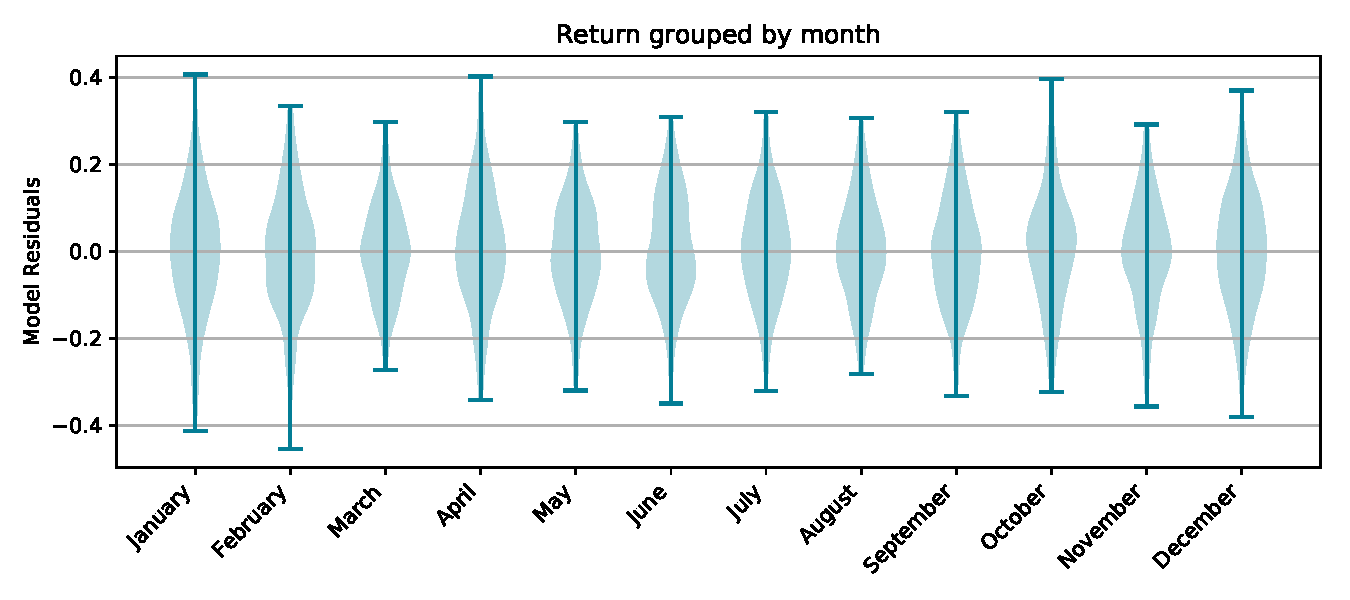
\includegraphics[width=\textwidth]{figures/regression/returns-per-month.pdf}
    \caption{Violin plot of preprocessed return values, denoted as model residuals, after taking the mean for each month and stock. The filled area visualizes the approximated data distribution along the vertical line}
    \label{fig:boxplot_seasons}
\end{figure}

Figure~\ref{fig:boxplot_seasons} shows the averaged model residuals for each month and stock. For every month the mean is not significantly different from zero but the standard deviation partially varies across the year. The lowest standard deviation is observed for the 467 values in March which equals 0.0998. The highest standard deviation 0.1266 is observed for January indicating a slightly increased uncertainty after the Christmas business. However, these result shows that there is no observable seasonality measured upon the mean monthly values. The same analysis was conducted for separate industries, too. While there is a significant seasonality visible on the original returns, they disappear after normalizing by the industry-wide mean, leading to similar zero-mean distribution as in Figure~\ref{fig:boxplot_seasons}.


\paragraph{Outliers}
Outliers are usually described as unexpected data points with an abnormal distance from the center of the data. The removal of such outliers is common but questionable practice since it can affect data properties. Unfortunately, there it is not easy to determine outliers in a non-parametric fashion for an arbitrary data distribution. A Student's $t$-distribution is most likely to fit the acquired data as pointed out before. Similar to the interquartile method for a normal distribution, an observation is seen as an outlier if it exceeds a chosen confidence interval. Suitable values for the distribution parameters (dimension of freedom, location and scale) are determined for each stock separately. Based on these parameters, the 99.5~\% confidence interval is calculated. Per definition, only 0.5~\%, i.e. five out of 984 observations, ought to be outside of this interval. On the preprocessed data, 199 stocks contain more than five outliers, but no more than seven.

\begin{figure}[!ht]
    \centering
    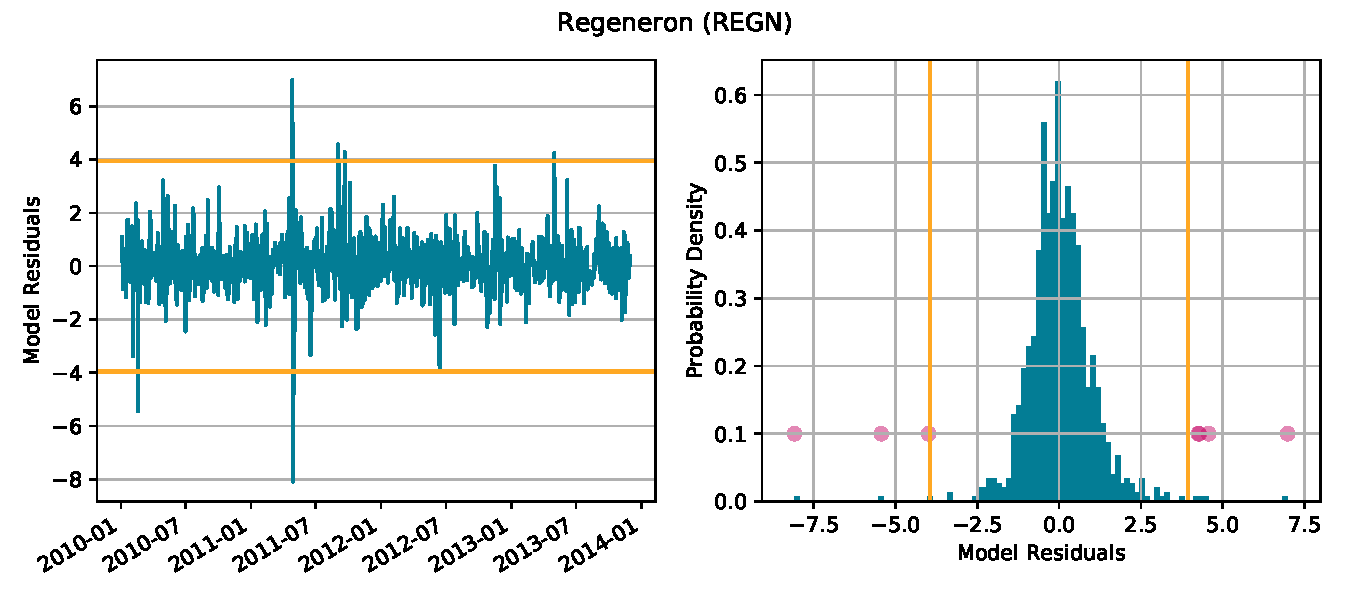
\includegraphics[width=\textwidth]{figures/regression/data-outliers-REGN.pdf}
    \caption{Preprocessed stock return and density histogram of those values for company \emph{Regeneron}. The orange line denotes the 99.5~\% confidence interval for a Student's $t$ distribution with four dimensions of freedom. On seven days an extreme value was observed which is denoted by a purple circle in the histogram on the right. The greatest two outliers can be observed for the 27th of April, 2011.}
    \label{fig:data_outliers}
\end{figure}

One stock with seven outliers is shown in Figure~\ref{fig:data_outliers}. At the 27th of April in 2011, the stock underwent a fast increase and decrease in value. This anomalous behaviour was caused by a successful study regarding a new drug for treatment of advanced colorectal cancer. The article \emph{\enquote{Regeneron, Sanofi Therapy Extends Lives of Colorectal Cancer Patients}} by Bloomberg, published in the evening of the 26th of April, reported these results.
 
Because removal or scaling down of unexpected extreme values, transforms the data in an unreasonable fashion and because it is not feasible to determine which data point should be considered actually unexpected, the outliers will not be treated different from the other data points. However, it is still worth mentioning that the number of outliers is not far above the expected value and therefore considered to not raise a sufficient influence on the data analysis.

% On the basis of a normal distribution, an observation would be to assumed to be an outlier if it falls below $Q1-1.5\times IQR$ or above $Q3+1.5\times IQR$, where $Q1$ and $Q3$ refer to the first and third quartile and $IQR$ to the interquartile range of the data.

% On the residuals, again the full analysis of characteristics was executed. In terms of stationarity, data distribution, heteroscedasticity, structural breaks and outliers no substantial change was observed.

\subsection{Time Series Correlation}
\label{subsection:cross_correlation}
Until this point, this section mainly focused on establishing statistical preconditions before it is possible to acquire cross-correlation. If the previous steps would be left out, the correlation would be much more likely to report erroneous results, e.g. spurious correlation. For calculating a bivariate correlation, Pearson's $r$ \eqref{formula:pearson_r}, will be used in the following.

% https://drive.google.com/file/d/1EKf_rly5OQ-oTts61HDeddYCwuBZLd1n/view

In order to make the danger of spurious correlation more tangible, Figure~\ref{fig:spurious_regression} shows an example for two stock prices which are not preprocessed. While the correlation on the plain stock prices appears very high with $r=0.96$, it is rather not existing at all after the preprocessing steps of differencing, transformation, normalization and modelling. This indicates that the first observed $r$ is high due to the autocorrelation of the both time series and their shared exogenous variable, i.e. the overall market performance.

\begin{figure}[!ht]
    \centering
    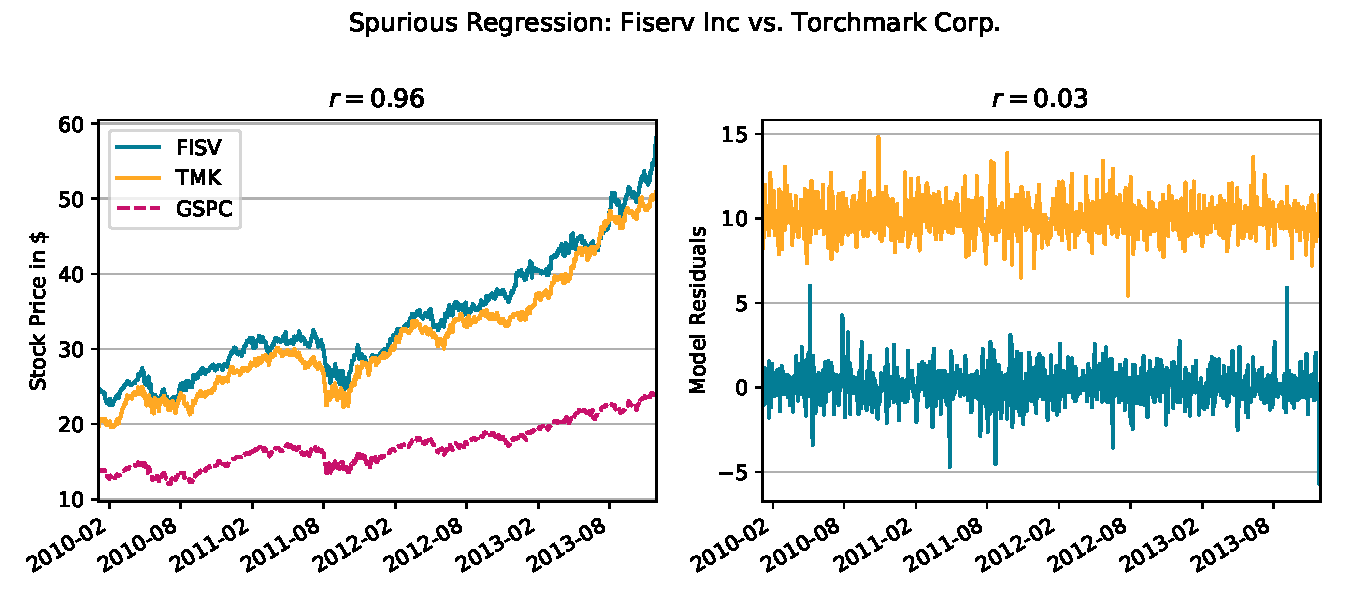
\includegraphics[width=\textwidth]{figures/regression/spurious-FISV-TMK.pdf}
    \caption{Data for the two companies \emph{Fiserv} and \emph{Torchmark}. The left plot shows the unmodified daily opening prices which revealed a Cross-Correlation of $r=0.99$. Additionally a scaled and shifted version of the market index is plotted. The right plot shows the same time series after properties like autocorrelation and heteroscedasticity were removed which led to $r=0.06$. For the sake of visibility, the orange time series is increased by 10.}
    \label{fig:spurious_regression}
\end{figure}

Even though $r$ is a very popular measure, it needs to be borne in mind that this measure does not account for nonlinear relationship which is not always a sufficient assumption. Therefore, the observed value might not fully reflect the real correlation but rather can be interpreted as an approximation. Since this limitation holds for all correlation values in this experiment, the values can fairly be compared to each other.

To see the impact of the several preprocessing steps, $r$ is calculated for each pair of stocks from four different phases. The distribution of $r$ for the original daily open prices, intraday returns, normalized returns and the residuals of the autoregressive models is visualized by violin plots in Figure~\ref{fig:steps-correlations-ind}. Because 467 stock prices are considered, there are 108.811 different pairs of stocks in total. With this high number of samples, the critical values for the 95~\% confidence interval are -0.006 and 0.006 respectively. Even for a more restrictive interval with $\alpha = 0.0001$, i.e. 99.99~\% confidence, the critical values are only -0.012 and 0.012 which for the whitened data in the last step still leads to 86~\% of all samples being significant. In consideration of this ever-present significance of correlation coefficients, the values are not evaluated by such confidence levels.

% Using the Student's $t$ distribution for the correlation coefficients

Except for autoregressive modelling, the distribution changes drastically with each preprocessing step. Initially, $r$ revealed a median of 0.48 and a great number of extreme values for the original stock prices. As the second distribution for price returns shows, this step does not tackle spurious correlation in a great manner. No pair of stocks is negatively correlated with each other since all stocks include the performance of the overall market or even the industry segment. After the exogenous impact was filtered out to a great extent, a more realistic distribution with a zero median can be observed. In general, stock prices share no more correlation with each other than the market performance and therefore reveal a coefficient close to zero. Relatively few stocks show a greater relationship which can be of a positive nature as well as of a negative nature.

\begin{figure}[!ht]
    \centering
    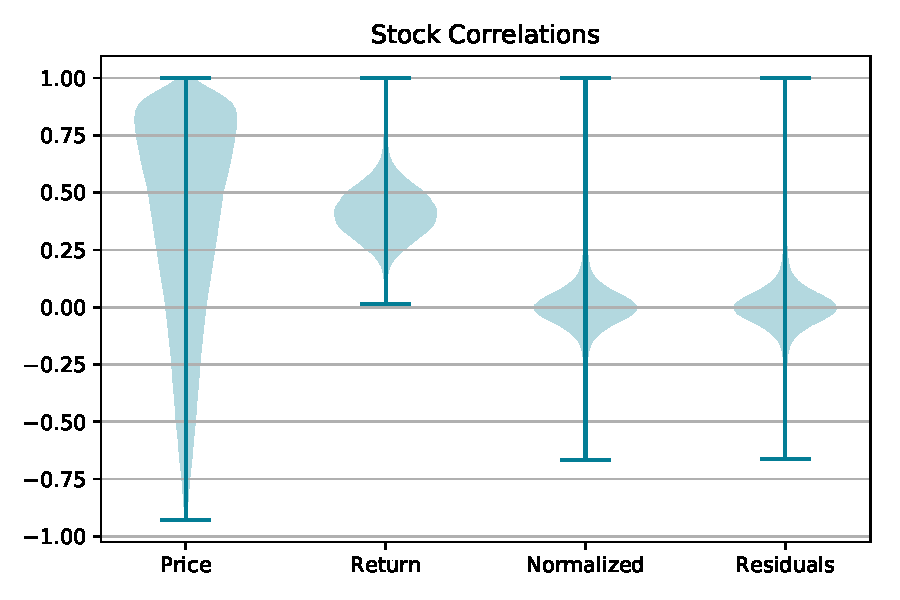
\includegraphics[width=0.8\textwidth]{figures/regression/steps-correlations-ind-norm.pdf}
    \caption{Violin plot of cross-correlation distributions for four main preprocessing steps. The filled area visualizes the approximated data distribution along the vertical line.}
    \label{fig:steps-correlations-ind}
\end{figure}

As mentioned in Section~\ref{subsubsection:processing:exogenous} the price returns can also be normalized by the S\&P~500 market index instead of separate industry means. For this alternative normalization method, the violin plots are shown in Figure~\ref{fig:steps-correlations-gspc}. Compared to the primary normalization by industry, the distribution is not located around zero but reveals a median of 0.2. Because all stocks are positively correlated with each other, this leads to the conclusion that not all exogenous influences are removed and therefore lead to spurious correlation. Concluding, the industry-wise normalization is preferable over market-wise normalization if one is interested in the cross-correlations among stocks from the same stock exchange.

\begin{figure}[!ht]
    \centering
    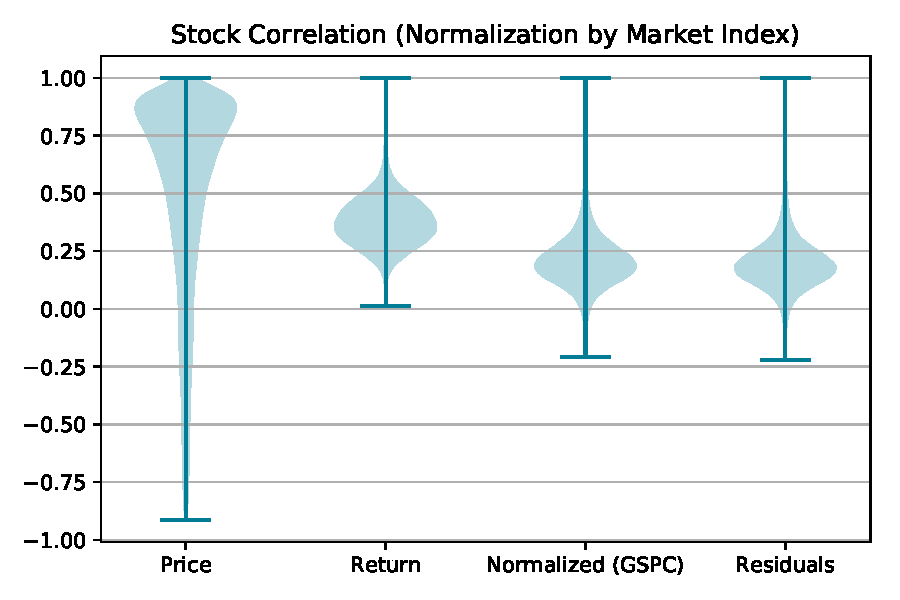
\includegraphics[width=0.8\textwidth]{figures/regression/steps-correlations-gspc-norm.pdf}
    \caption{Violin plot of cross-correlation distributions for four main preprocessing step with the normalization being adapted for market-wise instead of industry-wise normalization.}
    \label{fig:steps-correlations-gspc}
\end{figure}


\paragraph{Correlation Graph}

In order to visualize and inspect the calculated cross-correlations, a graph is defined and visualized in Figure~\ref{fig:graph-correlations}. As stated earlier in this section, there is a tremendous number of significant correlations. If all these correlations would be considered, the plotted graph would become unmanageable. Instead, the 99.9th percentile of all absolute correlation coefficients is calculated which equals 0.3688. Only positive or negative values outside of this percentile are considered for visualization. This leads to 109 correlations among 123 different stocks from all industry sectors. A node's size is determined respectively to its total revenue in 2010 in order to indicate its importance.

On this rather small and incomplete graph, individual nodes, connections and communities in the form of subgraphs can be further examined. It should be noted that the graph consists of the most extreme values and therefore is not a representative sample for the entire graph which would reveal an unmanageable number of edges.

\begin{figure}
    \centering
    \begin{subfigure}{\textwidth}
        \centering
        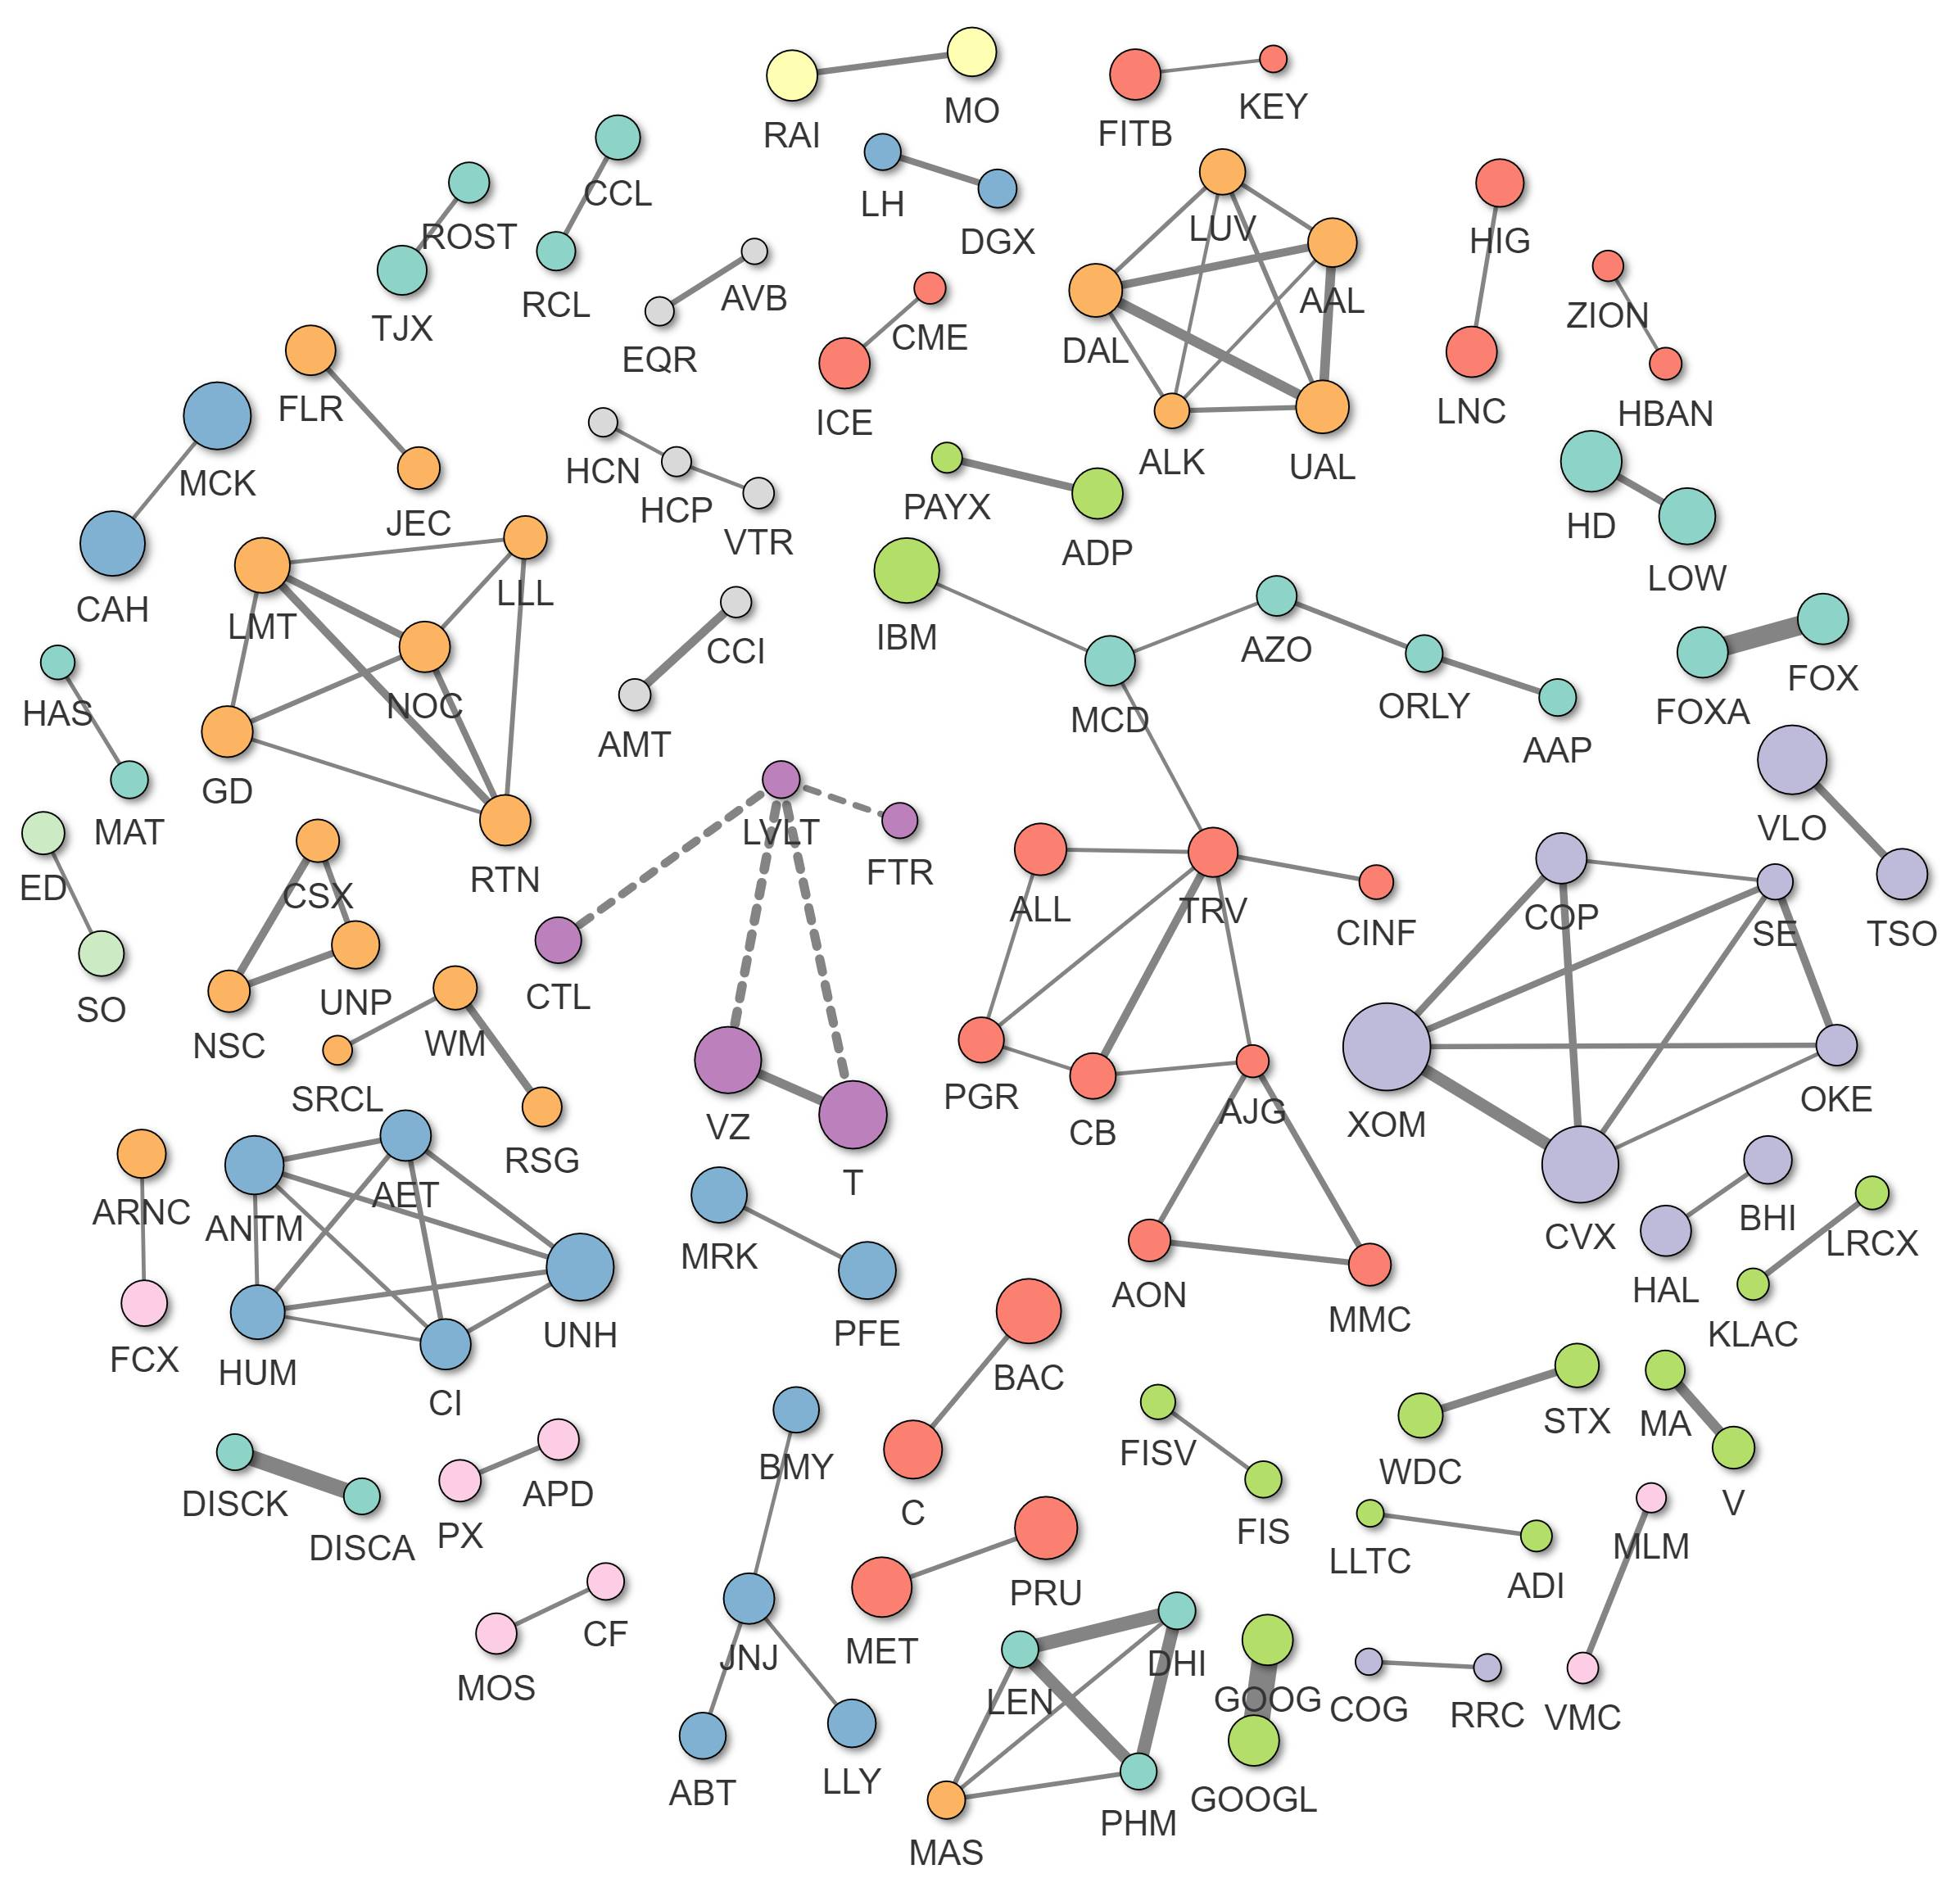
\includegraphics[width=\textwidth]{figures/regression/graph-corr-resid-999-42-with-neg.jpg}
    \end{subfigure}
    \vfill
    \begin{subfigure}{\textwidth}
        \centering
        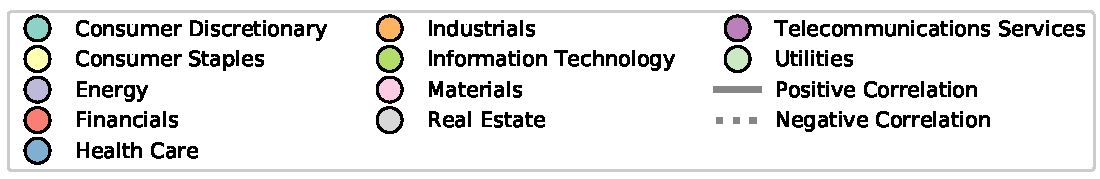
\includegraphics[width=\textwidth]{figures/graph-legend.pdf}
    \end{subfigure}

    \caption{Graph of the 109 greatest cross-correlations among stocks. Each node represents one stock which is labeled by the company's ticker symbol and coloured by the regarding industry section. Which color belongs to which industry is provided by the legend below. The node's size is determined by the total revenue for this company. Each edge between two nodes represents the cross-correlation $r$ between those stocks. More extreme values are indicated by a thicker edge and negative values by a dashed line.}
    \label{fig:graph-correlations}
\end{figure}

As indicated by the node colors, a large proportion of high correlations are observed among companies belonging to the same industry sectors. Only eight edges between two different sectors are present in this visualization. In terms of inter-industry connections, the node \emph{MCD} (\emph{McDonald's Corp.}) in the center of the graph is the strongest one since it is connected to nodes from three different industries. Investigation by financial news did not reveal an underlying relationship with the connected companies. Instead, this stock appears to be an appropriate strong representative component of the market performance and therefore is strongly linked to other important representative components like \emph{IBM} (\emph{International Business Machines}).

From the 109 edges selected for the graph, only four represent a negative correlation which all originate from the industry sector \emph{Telecommunications Services}. Further, it should be noted that there a three companies for which each one compromises two stocks. The reasoning for this is given in the previous Section~\ref{section:data}. Because two stocks of the same company are almost equal. these three correlation pairs reveal the highest $r$.

As denoted previously, this graph is not representative for the meaning of the measured cross-correlations. In order to examine this feature's usability, the final evaluation in Section~\ref{section:evaluation} will conduct a comparison with the extracted business relationships which are introduced in the following section.




% \begin{itemize}
%     \item Describe graph figure. Which correlation where chosen (99.9~\% Percentile: 0.3688, 123 nodes, 109 edges (incl 4 neg), 11 industries)
%     \item Collect insights: Only 8 edges between comps with different industry. Concluding, industry-correlation still exists
%     \item Not whole industries are connected but only pairs within industries giving evidence more meaningful relationships than just being in the same industry.
%     \item \emph{McDonald's Corp.} (node \emph{MCD} in the center of the graph) is the strongest connected node across several industries. Since investigation did not reveal an underlying relationship with the connected companies, this stocks instead appears to be an appropriate strong representative component of the market performance.
%     \item{Pairs of two stocks belonging to the same company are not removed}
% \end{itemize}




% \todo{Optional: Mutual Information, Cointegration, Granger Causality}

%%% Inspecting Cross-Dependencies
% Look into Dean2015 for more insights
% Calculate cross-correlation between residuals of stocks.
% Visually inspect change of cross-correlations over years? (like Mantegna)
% -> Inspect normalized MI and Pearson's r (as done by Dionisio)

% Cointegration & Causality Analysis
% Paper using Cointegration (Johansen Test): Kosapattarapim2017 https://drive.google.com/file/d/1wMcZlYGR69HT-JAH5382FIyfS4yh5gCC/view
% Paper using Granger Causality: Bollean2011 https://drive.google.com/file/d/1hv6CoM-_GnhDtVOGjhu-N3btCAIaA1an/view
% BDS (Bock, Dechert and Scheinkman[Hsieh 1989]) test (Dionisio2004) to test if variables are nonlinear independent
% Test for Unit Root, Cointegration, Granger Causality (bidir gc vs. simultaneity)



% Inspect correlation and prices in general for one specific quarter (e.g. 2011/02 appears to be bad for Energy)




% Prediction:

% For experiments incorporating both datasets only the overlapping time period is used. Training: 2010 - 2013 (1st half), Test: 2013 (2nd half). Test is left out up to the final evaluation. The training set will be splitted into chunks to apply cross-validation (as pointed out by Hsu et al) along time series (e.g. Li et al 2014).
% How to upsample stock prices?
% Stratified sampling to ensure similar class distribution in train, val & test ?
% Evaluate good class threshold
% Evaluate good prediction frame size



%%% Links Stack
% Links about regression steps
% Example 1: Regression Diag http://songhuiming.github.io/pages/2016/12/31/linear-regression-in-python-chapter-2/
% Example 2: Regression Diag https://www.statsmodels.org/0.8.0/examples/notebooks/generated/regression_diagnostics.html
% Example: ARIMA & GARCH modelling http://www.blackarbs.com/blog/time-series-analysis-in-python-linear-models-to-garch/11/1/2016
% Example 3: Testing for Unit root and cointegration
% https://pdfs.semanticscholar.org/7ce6/2a0c7f6dab85f264a5403bf9b99a0f20a156.pdf
% Example: Apply ARMIA vs GARCH  https://scialert.net/fulltextmobile/?doi=jas.2011.1129.1135
% Methodology for ARIMA, GARCH, etc.: https://sci-hub.se/10.2139/ssrn.2540535
% Example 1: Regression Model https://www.kaggle.com/benjibb/prototype-gspc
